\begin{figure}
    \centering
    
        
        \begin{tabular}{c c c c}
            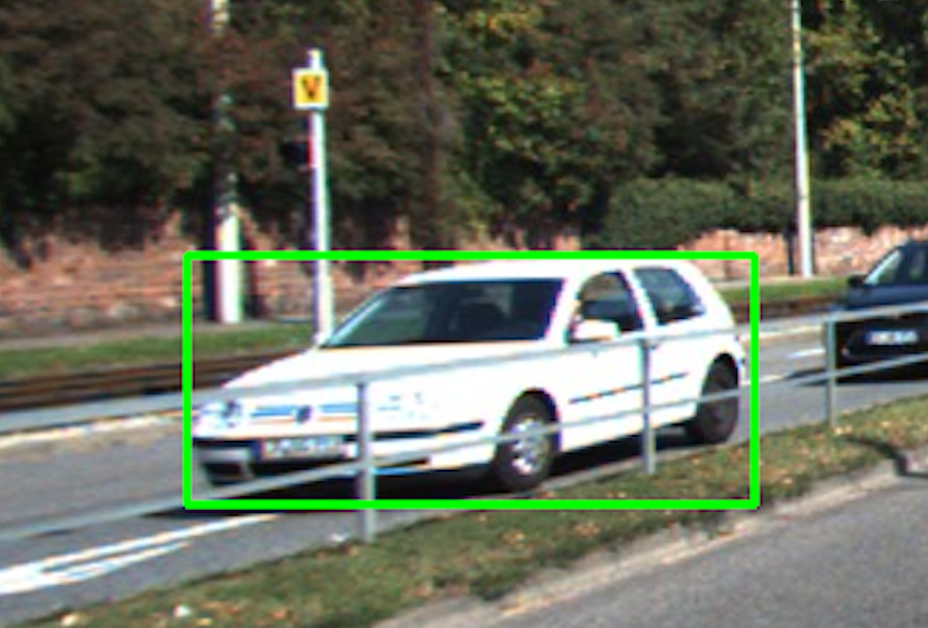
\includegraphics[width=0.25\textwidth]{figures/method/output_examples/rgb-1.png} &
            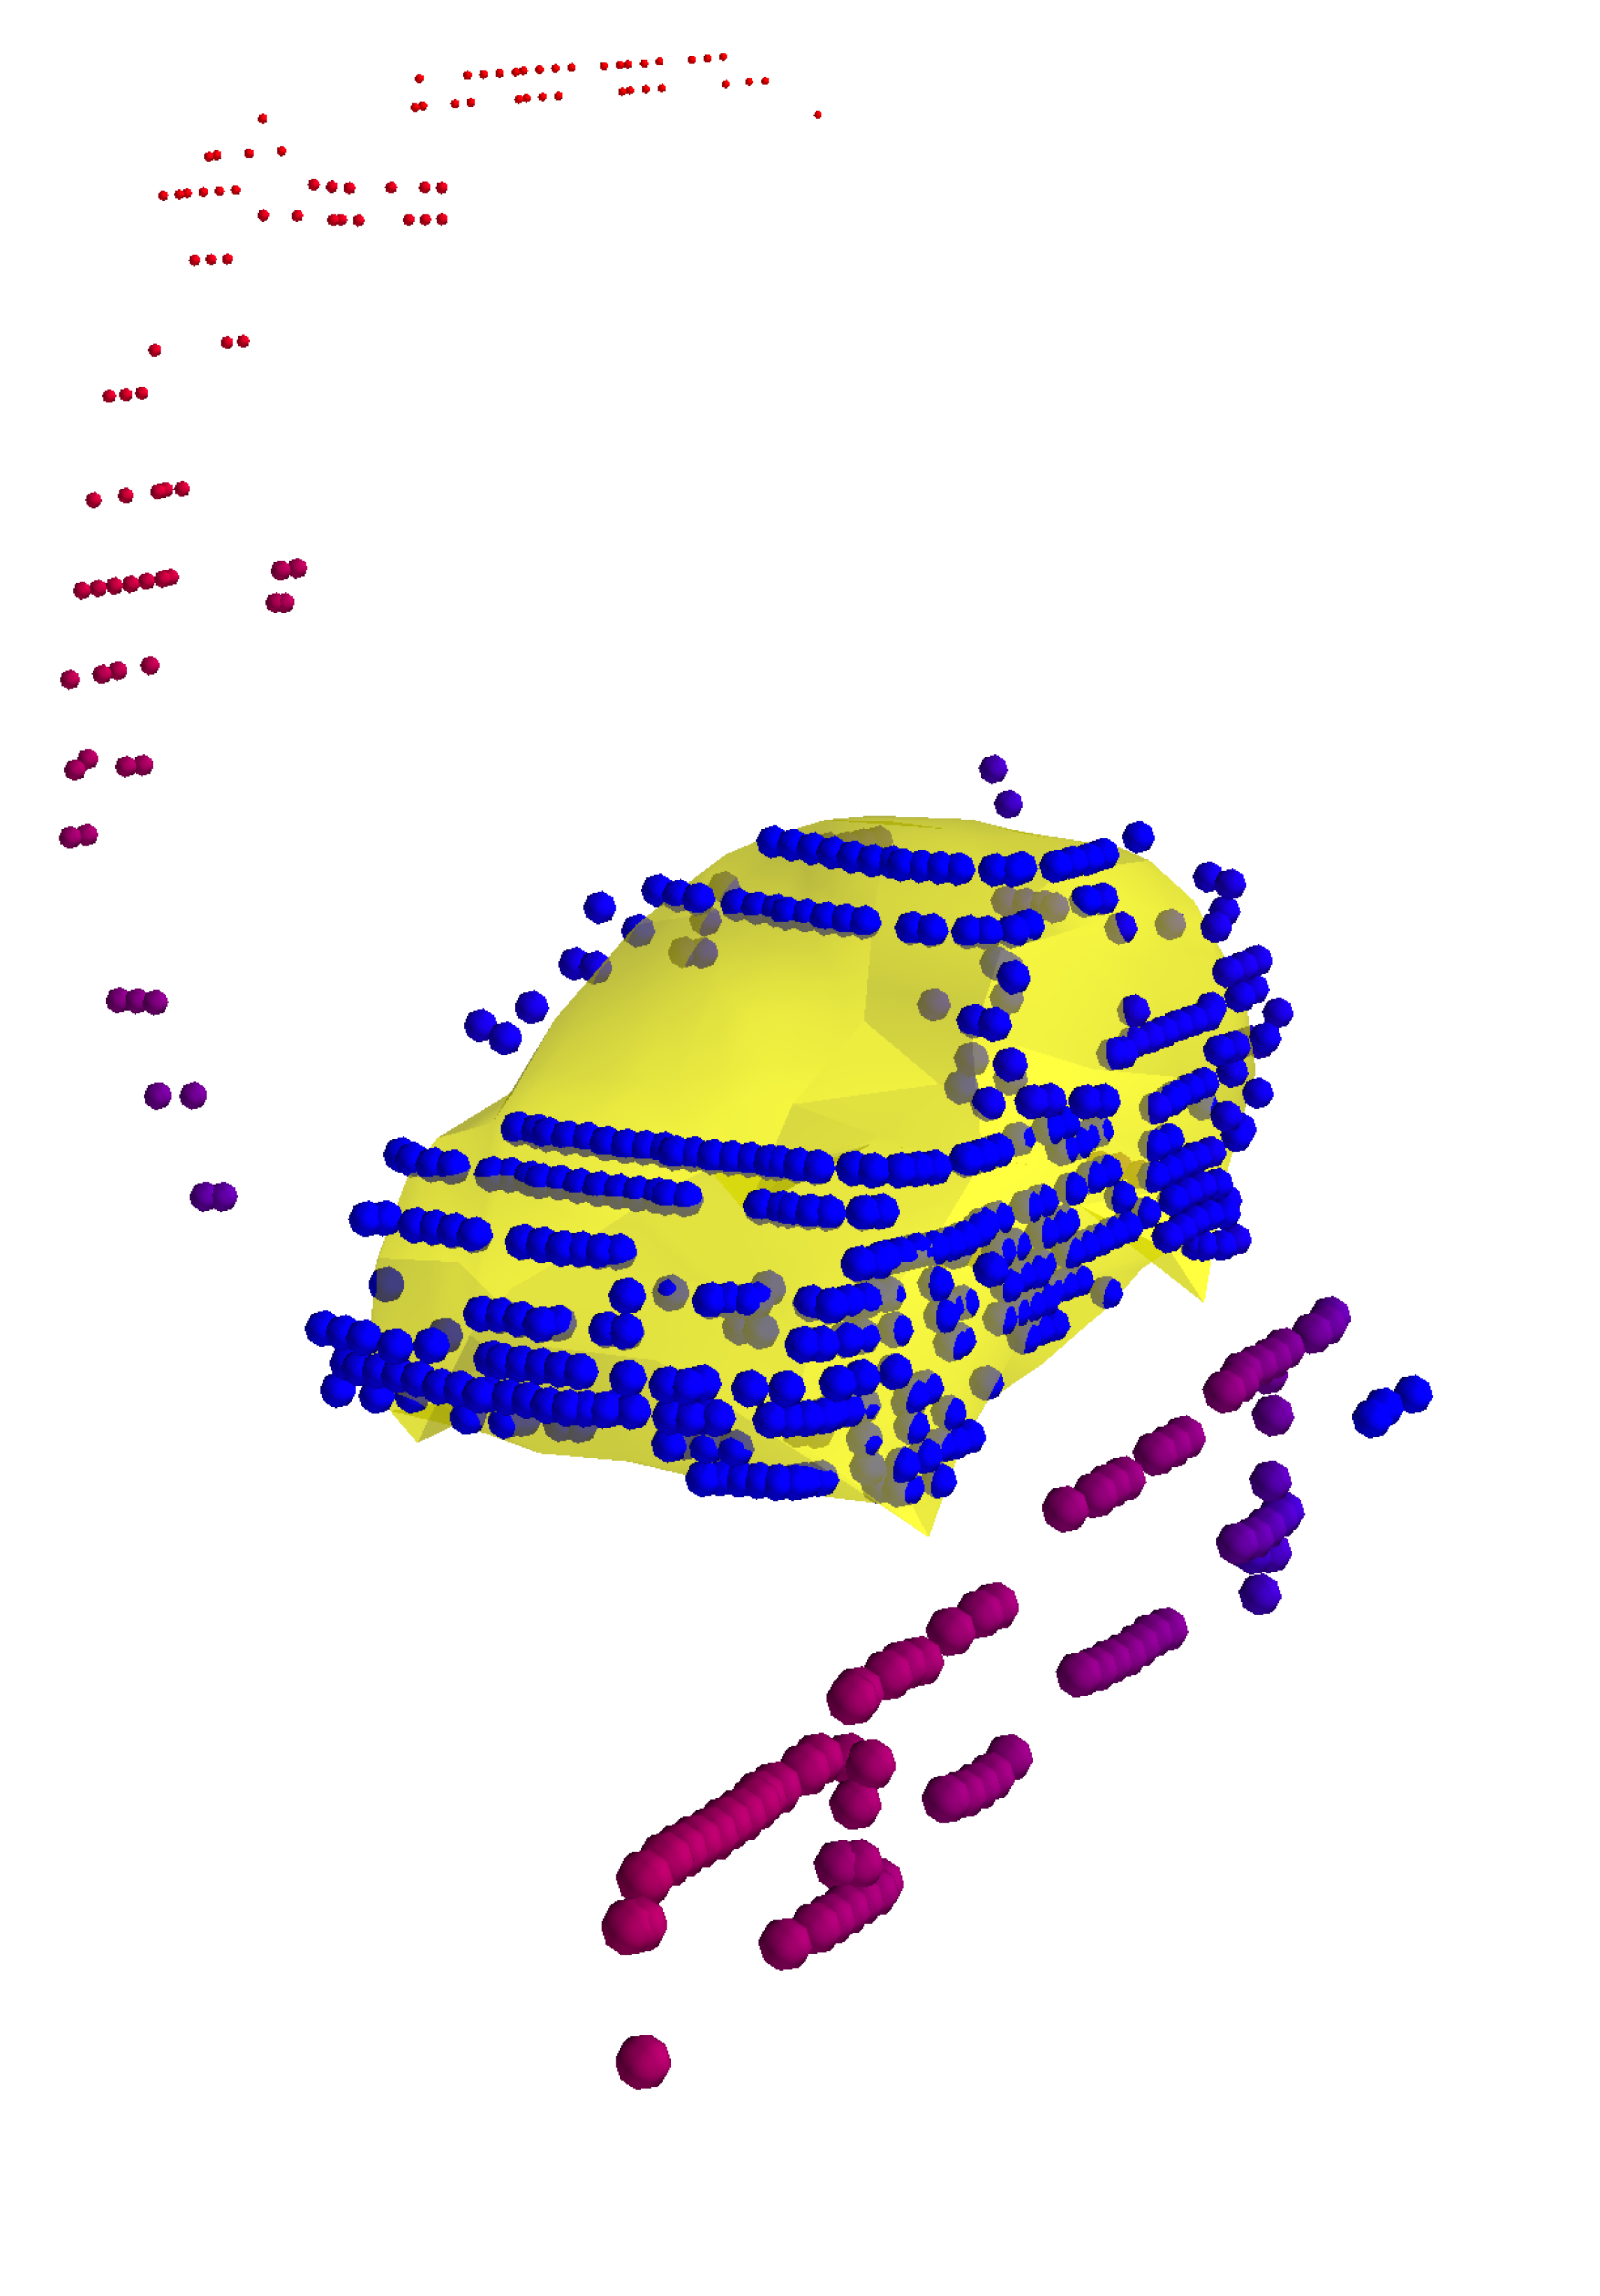
\includegraphics[width=0.25\textwidth]{figures/method/output_examples/pcd-1.png} &
            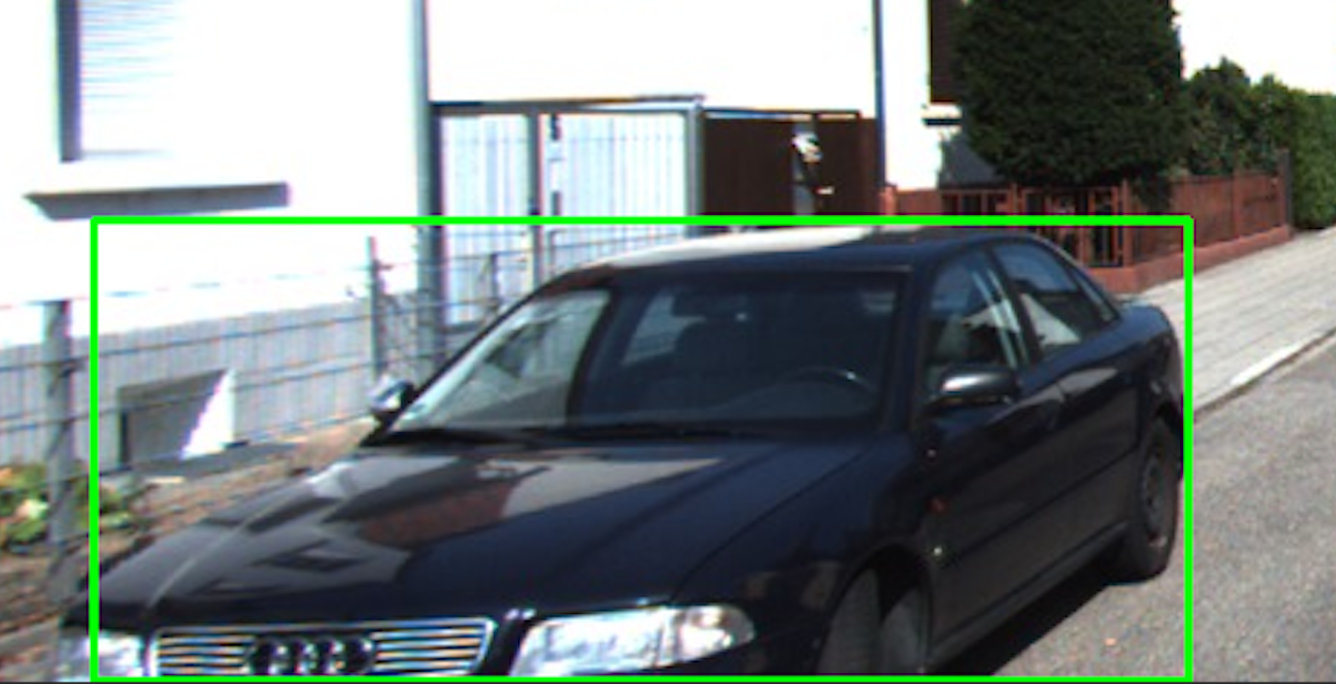
\includegraphics[width=0.25\textwidth]{figures/method/output_examples/rgb-2.png} &
            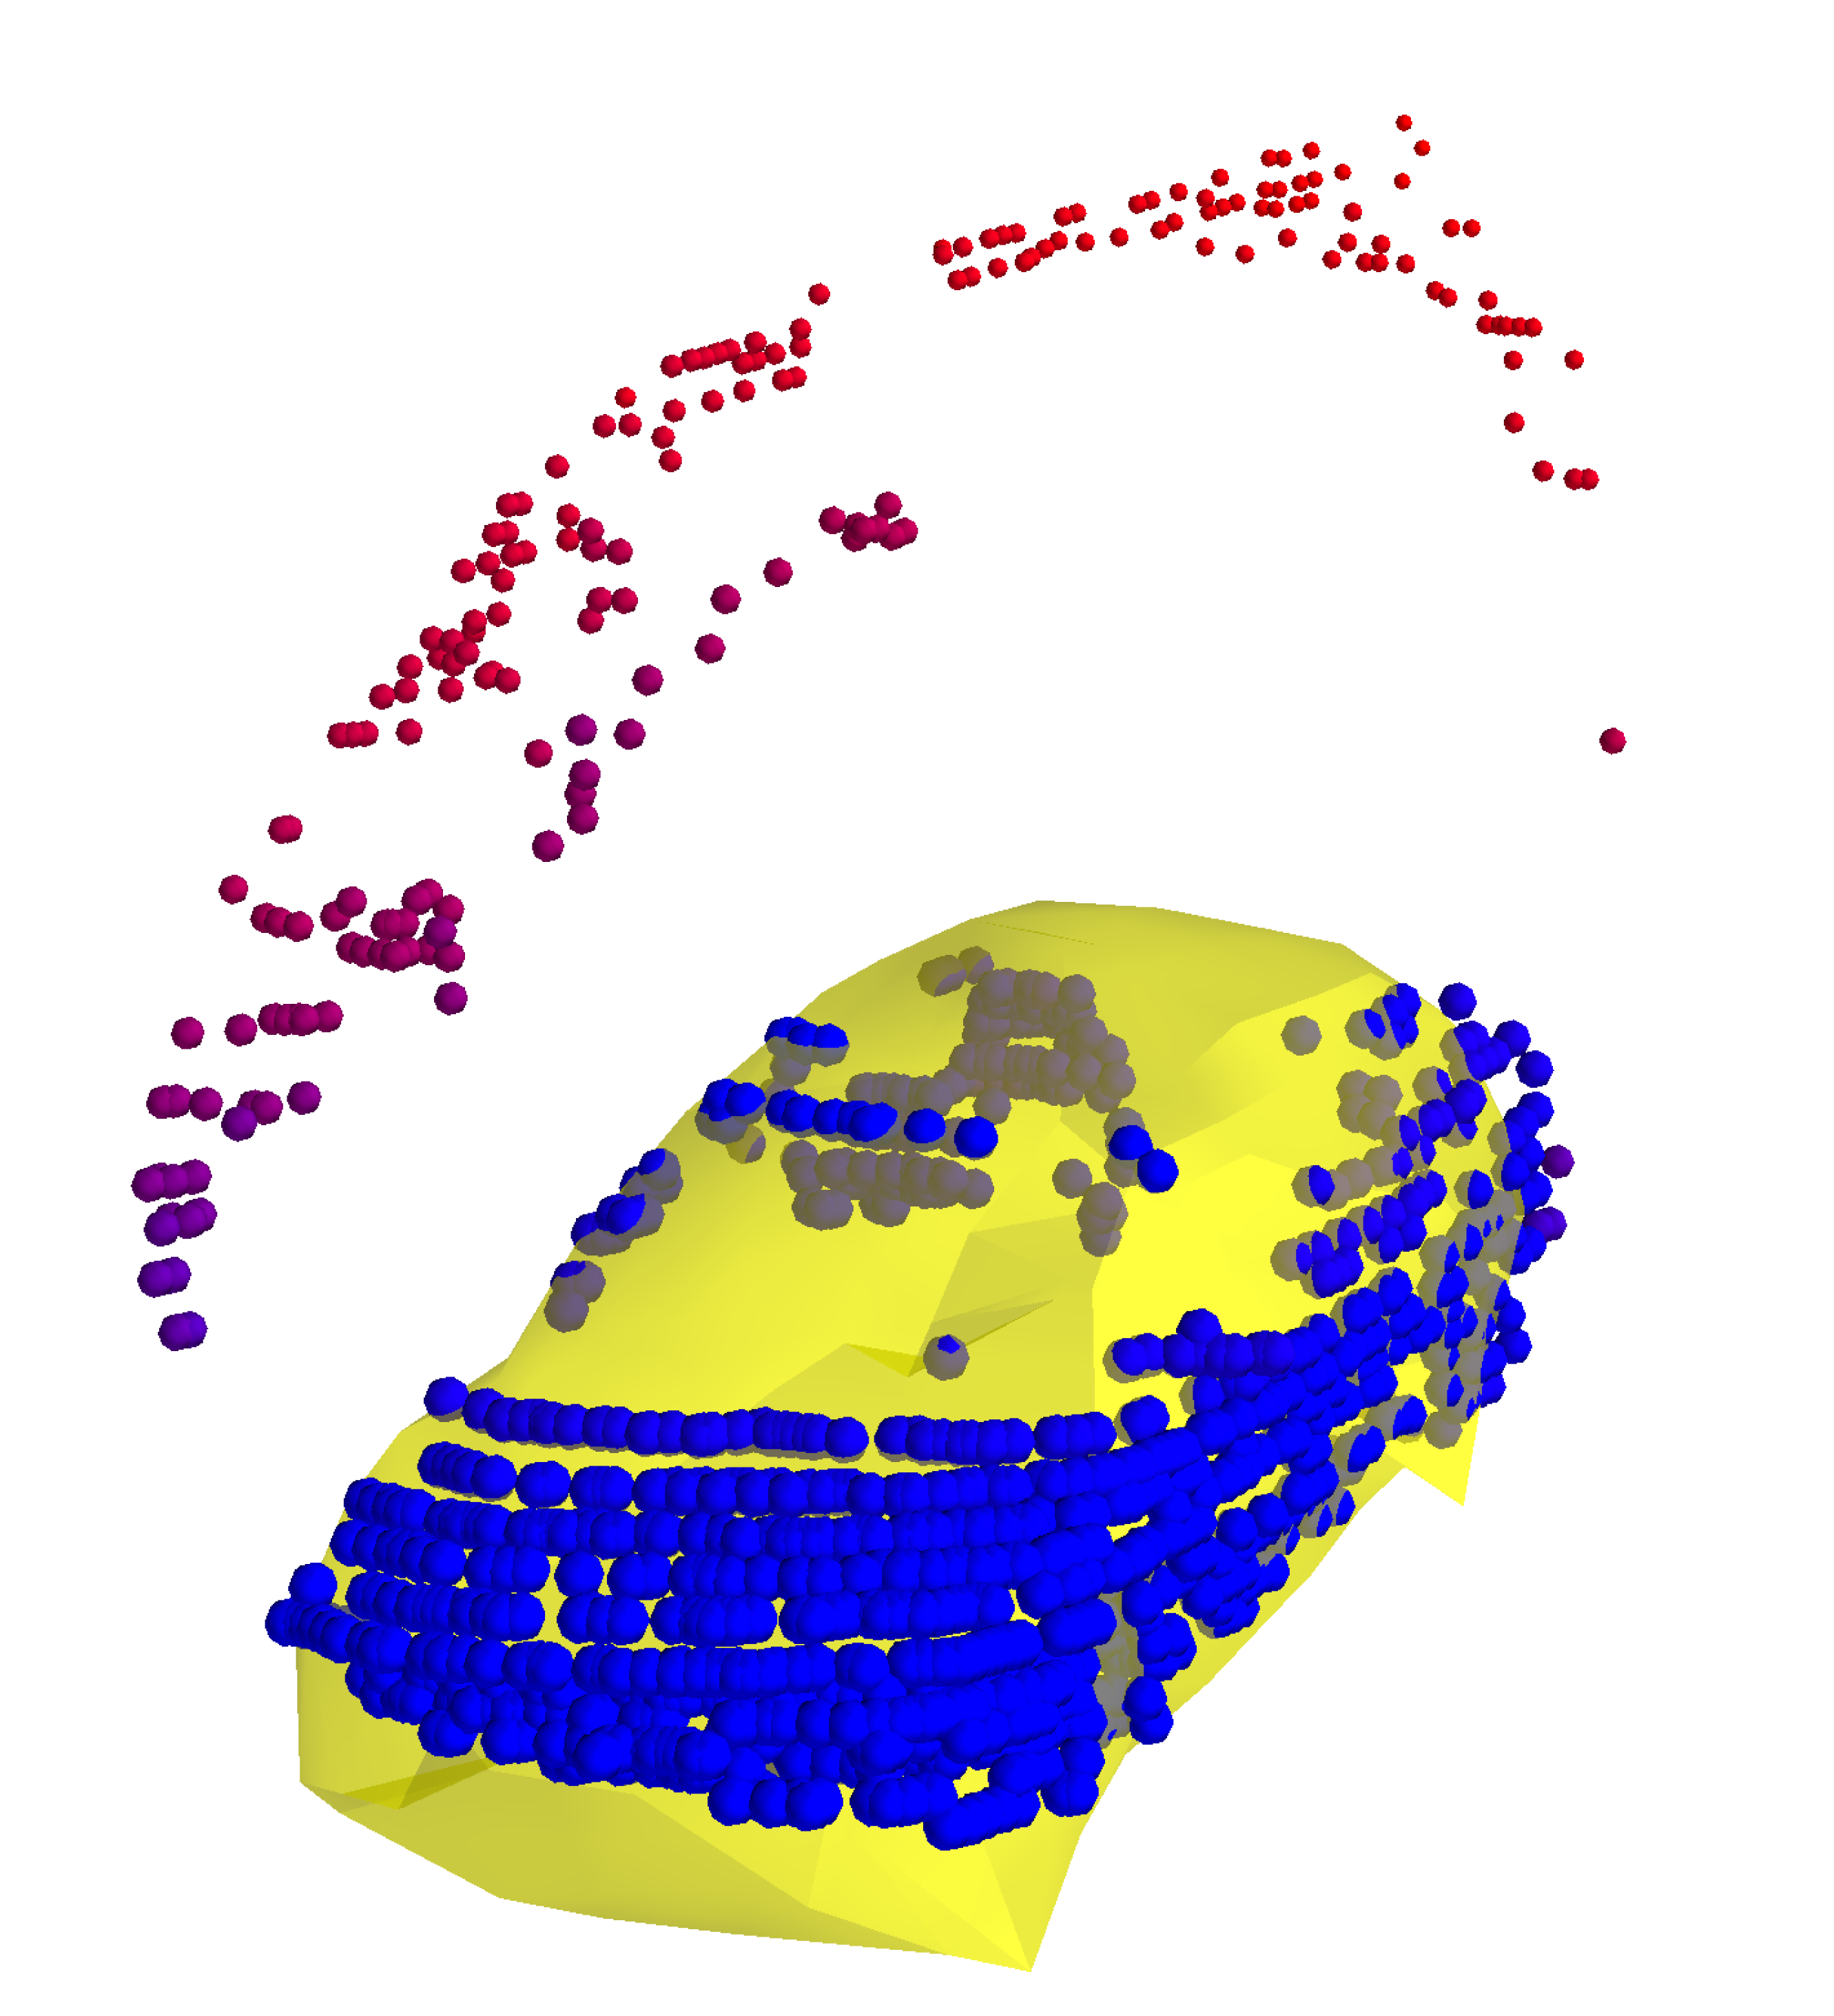
\includegraphics[width=0.25\textwidth]{figures/method/output_examples/pcd-2.png}
        \end{tabular}
        \caption{Even after removing LiDAR points which do not project into the 2D instance mask we still have a large number of outliers, mainly caused by partial occlusions and points at the boundary where 2D masks struggle. The $\sigma^2(\X)$ value predicts the relevance of a point to the cars location with blue points having low values with a gradient to red for higher values which suggests the point is an outlier.}
    \label{fig:my_label}
\end{figure}